\chapter{System use cases}
\label{system-uc}

\par To maintain the overview of the system use case diagram, the diagram was
split in 2 diagrams (figures \ref{fig:system-use-case-diagram1} and
\ref{fig:system-use-case-diagram2}. The functionality for logging in and off
(figure \ref{fig:system-use-case-diagram2})was separated in a second diagram
because of the complexity of the actors hierarchy.

\begin{figure}[H]
	\begin{centering}
		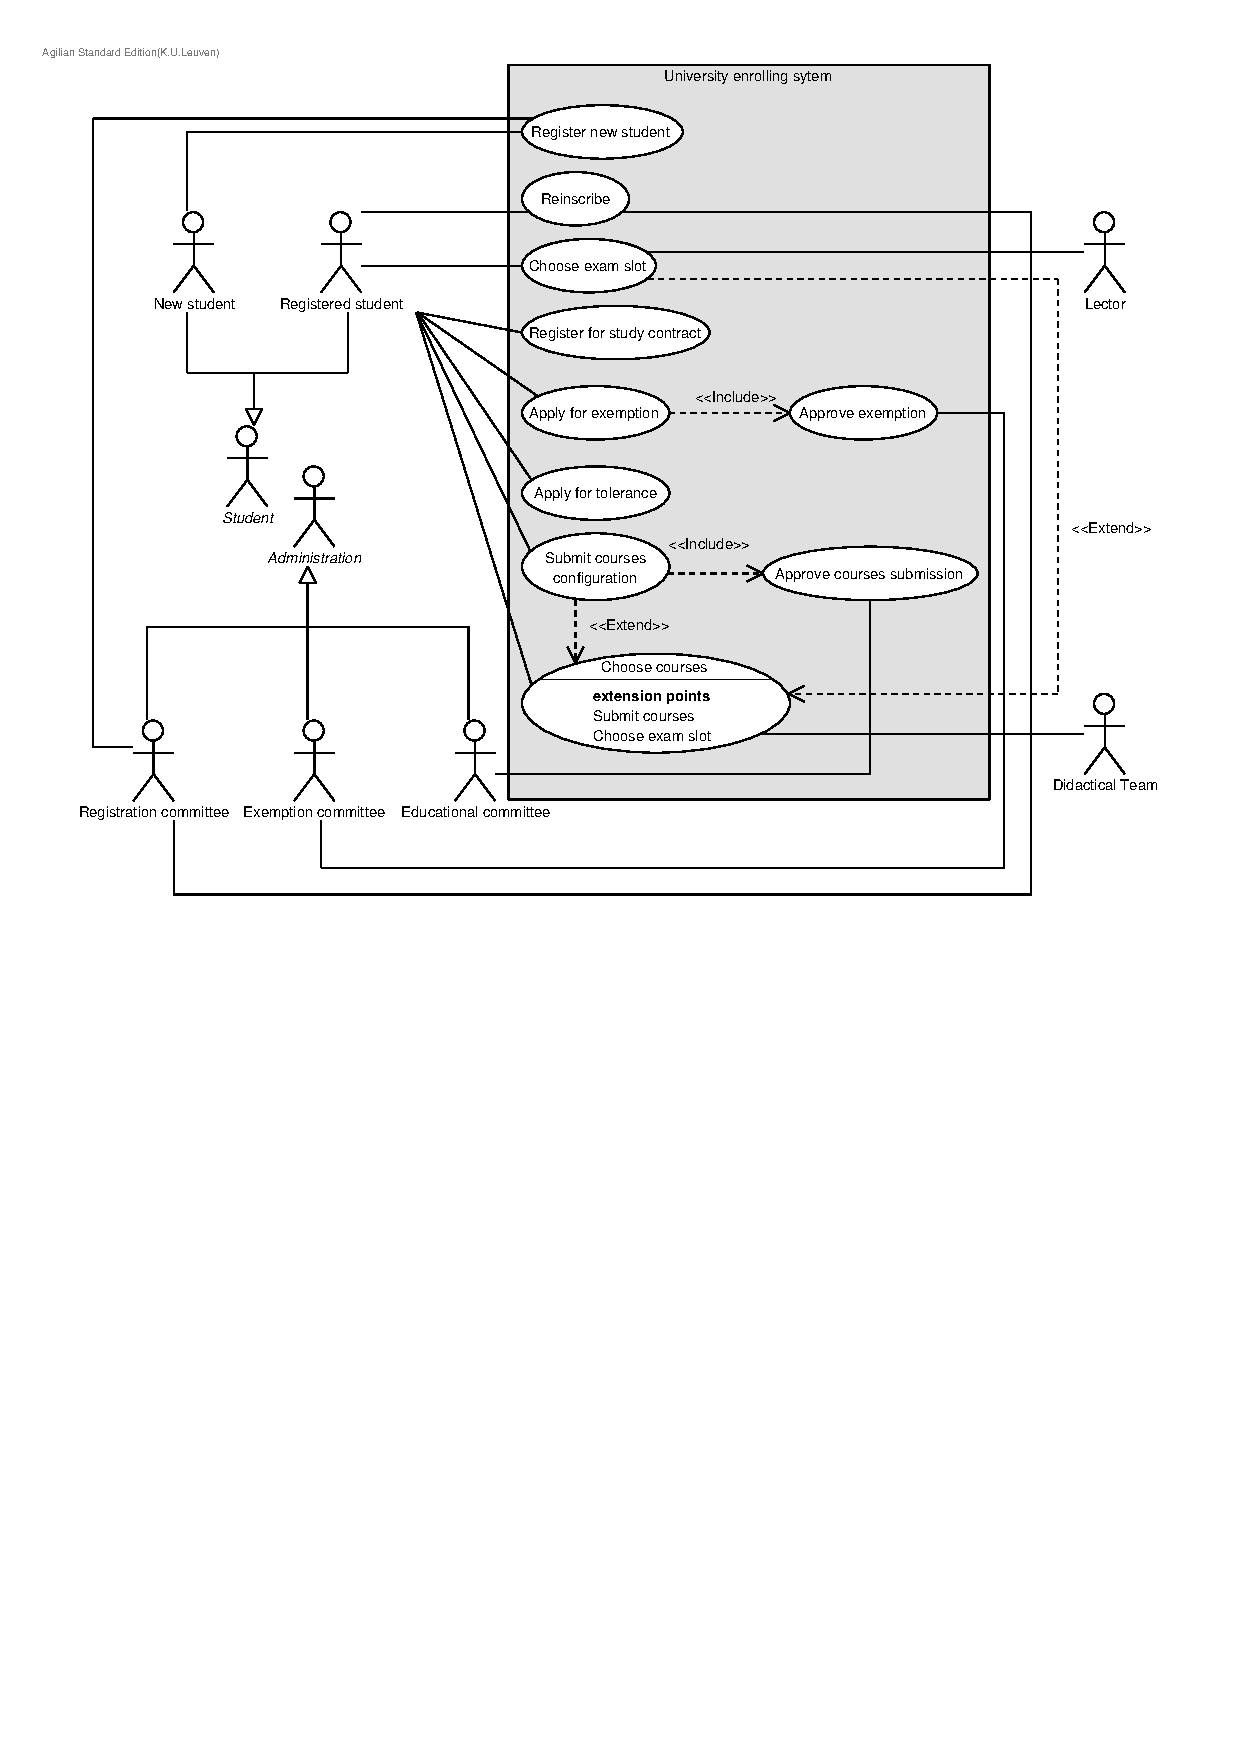
\includegraphics[width=\textwidth]{figs/system-use-case-diagram1.pdf}
		\caption{Part 1 of the system use case diagram}
		\label{fig:system-use-case-diagram1}
	\end{centering}
\end{figure}

\begin{figure}[H]
	\begin{centering}
		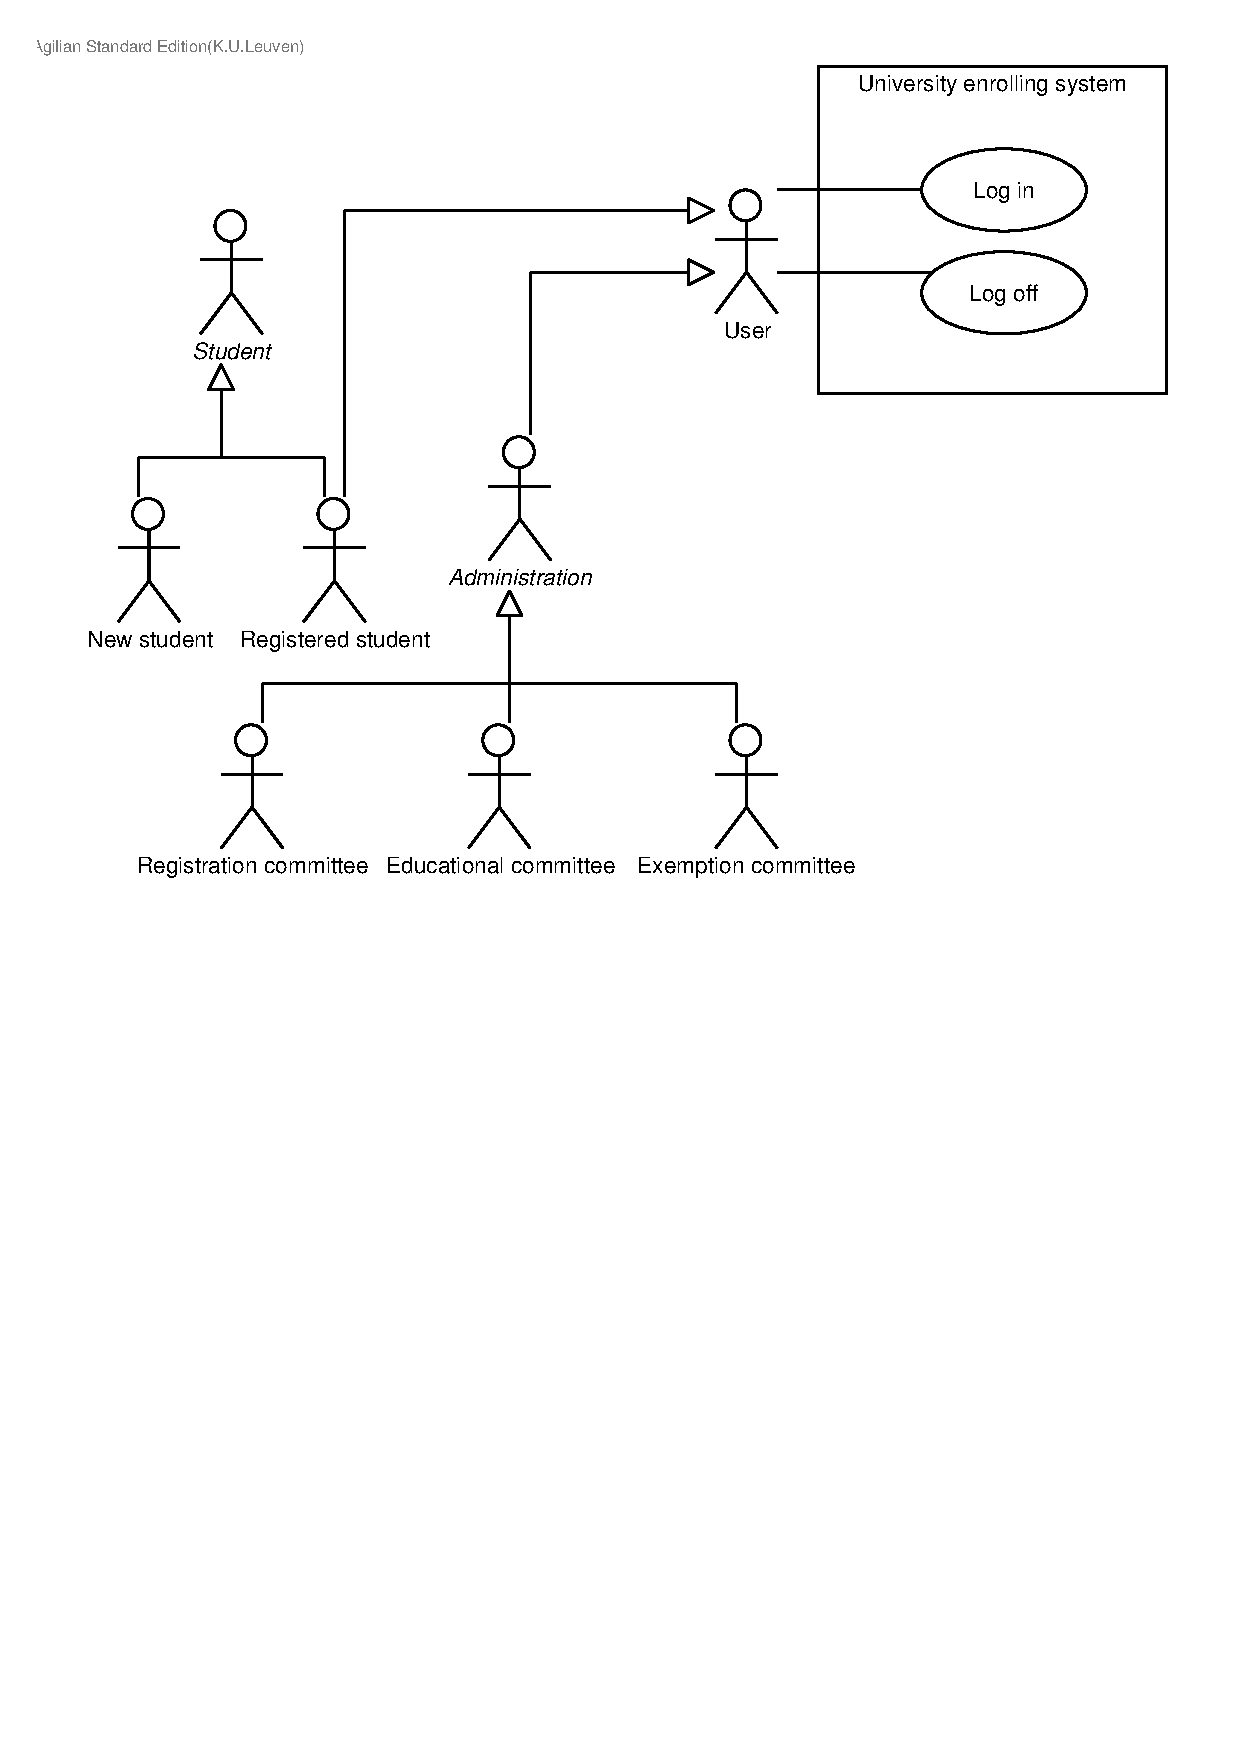
\includegraphics[width=\textwidth]{figs/system-use-case-diagram2.pdf}
		\caption{Part 2 of the system use case diagram}
		\label{fig:system-use-case-diagram2}
	\end{centering}
\end{figure}

\section{Register new student}
\label{register-new-student}

\begin{description}
	\item[Business Event Description] \
	\par A student wants to register at the Wellington
	University
	\item[Business Use Case Name] \
	\par Register new student
	\item[Triggering business event] \
	\par A student wants to register at the Wellington
	University. He is completely new and hasn't studied at Wellington before. He
	goes to the student administration building of Wellington University to make
	his inscription.
	\item[Preconditions] \ 
	\begin{itemize}
		\item Student hasn't yet studied at Wellington University.
		\item Student has a high school degree.
	\end{itemize}
	\item[Active stakeholders] \ 
	\begin{itemize}
	  	\item Student: wants to study at Wellington University.
		\item Registration employee: needs to complete the inscription of the student.
	\end{itemize}
	\item[Interested stakeholders] \ 
		\begin{itemize}
		  \item Board of the university: interested in new students.
		\end{itemize}
	\item[Normal business flow] \
	\begin{enumerate}
	  	% 1
	  	\item The student goes to the student administration building of Wellington
	  	University.
	  	% 2
	  	\item The student hands over the required information at the registration
	  	desk: home address, residence address, phone numbers, birth date, passport
	  	picture, register number, diplomas, if necessary evidence of matriculation.
	  	% 3
	  	\item The registration employee checks if the provided information is enough
	  	and is correct.
	  	% 4
	  	\item The registration employee makes the right documents: invoice,
	  	inscription attest.
	  	% 5
	  	\item The registration employee prints the student card with a unique
	  	student number and the passport picture of the student on it.
	  	% 6
	  	\item The registration employee grabs a few other documents like some
	  	folders and a free buss card.
	  	% 7
	  	\item The registration employee hands all these documents and student card
	  	over to the student.
	  	% 8
	  	\item The student accepts all these documents and is now successfully
	  	inscribed to Wellington University.
	\end{enumerate}
	\item[Alternative business flow] \ 
	\begin{description}
  		\item[3a] The registration employee notices that some documents are missing
  		because the student has forgotten to bring them.
  		\begin{enumerate}
  			\item The registration employee makes the student aware that he/she
  			can't be inscribed without these documents.
  			\item The student leaves to retrieve the missing documents.
  			\item The student returns at the student administration to restart his/her
  			inscription.
  			\item Go to normal flow 4.
		\end{enumerate}
	\end{description}
	\item[Exception business flow] \
	\begin{description}
		\item[3a] after having checked the information provided by the student, the
		registration employee notices that some documents are missing. This time not
		because the student has forgotten them, but because the student just doesn't
		have these documents (high school diploma, evidence of having passed a
		matriculation, \ldots).
		\begin{enumerate}
		  \item The registration employee makes the student aware that he/she can't be
		  inscribed without these documents.
		  \item The student leaves and can't be inscribed until he obtains the missing
		  documents.
		\end{enumerate}
	\end{description}
	\item[Outcome (postcondition)] \
	\par The student is now fully inscribed at Wellington University and has
	received all the according documents, folders, buss card and student card.
\end{description}

\section{Log in}

\begin{description}
	\item[Name] \
		\par Log in
	\item[Short description] \ 
			\par The user wants to access to the online study board. He therefore uses
			his credentials (e.g. student number and corresponding password in case
			the user is a student). 
	\item[Trigger] \ 
			\par The user decides he wants to access the online study board.
	\item[Primary actor(s)] \ 
		\begin{itemize}
		  \item User
		\end{itemize}
	\item[Secondary actor(s)] \ 
		\par None
	\item[Preconditions] \ 
	\begin{itemize}
		\item The user is either a registered user at the Wellington university and
		hence possesses a valid student number and password or he is an administration
		associate.
	\end{itemize}
	\item[Normal flow] \ 
	\begin{enumerate}
	  	% 1
	  	\item The user can signal at any time that he wants to access to the online
	  	study board.
	  	% 2
	  	\item The user provides his user credentials (e.g. student number and
	  	password).
	  	% 3
	  	\item The system validates the user credentials.
	  	% 4
	  	\item The system gives the user access to the functionality of the online
	  	study board system that corresponds with his role.

	\end{enumerate}
	\item[Alternative flow] \
		\par None
	\item[Postcondition(s)] \ 
		\par The user is logged in and has access to the functionality that
		corresponds with his role.
	\item[Exception(s)] \
	\begin{description}
		\item[3a] If the user id is unknown, then
		\begin{enumerate}
		  \item The system informs the user about the error.
		  \item The system invites the user to try again.
		  \item The UC flow continues at step 2.
		\end{enumerate}
		\item[3b] If the password is incorrect, then
		\begin{enumerate}
		  \item The system informs the user about the error.
		  \item The system invites the user to try again.
		  \item The UC flow continues at step 2.
		\end{enumerate}
	\end{description}
\end{description}


\section{Register for study contract}

\begin{description}
	\item[Name] \
		\par Register for study contract
	\item[Short description] \ 
			\par The student wants to register for a study contract, hence he has to
			specify the necessary information.
	\item[Trigger] \ 
			\par The student wants to register for a diploma contract and decides to take
			the necessary steps.
	\item[Primary actor(s)] \ 
		\begin{itemize}
		  \item The student
		\end{itemize}
	\item[Secondary actor(s)] \ 
		\par None
	\item[Preconditions] \ 
	\begin{itemize}
		\item The student is logged in at the online study board.
	\end{itemize}
	\item[Normal flow] \ 
	\begin{enumerate}
	  	% 1
	  	\item The student navigates to the registration page.
	  	% 2
	  	\item The system displays the registration page.
	  	% 3
	  	\item The student indicates that he wants to register for a diploma
	  	contract.
	  	% 4
	  	\item The student selects the right program. This includes the actual
	  	program as well as the phase.
	  	% 5
	  	\item The student verifies that he selected the correct program and submits.
	  	% 6
	  	\item The system verifies that the student can indeed follow the specified
	  	study program.
	  	% 7
	  	\item The student is now registered for the program.
	\end{enumerate}
	\item[Alternative flow] \
	\begin{description}
		\item[3a] The student indicates that he wants to register for an exam
		contract, resume at step 5 in the normal flow.
		\item[3b] The student indicates that he wants to register for a credit
		contract, resume at step 5 in the normal flow.
	\end{description}
	\item[Postcondition(s)] \ 
	\begin{itemize}
		\item The student is now registered for the specified study program. The
		Wellington university is aware that a new student is subscribed to one of
		their study programs.
	\end{itemize}
	\item[Exception(s)] \ 
	\begin{description}
		\item[6a] if the student's submitted program is a credit or exam contract and
		the student has already registered for another contract of that same type
		within the same faculty, then
		\begin{enumerate}
		  \item The system rejects the registration
		  \item The system presents the option to register for another study program
		  (and hence return to step 3 in the normal flow) or end the registration.
		\end{enumerate}
		\item[6b] if the student's submitted program is about a phase X where the
		student did not yet complete phase X-1, then
		\begin{enumerate}
		 	\item The system rejects the registration
		 	\item The system presents the option to register for another study program
		 	(and hence return to step 3 in the normal flow) or end the registration.
		\end{enumerate}
		\item[6c] if the student's submitted program is about a master where the
		student did not yet complete the preceding bachelor, then.
		\begin{enumerate}
		 	\item The system rejects the registration
		 	\item The system presents the option to register for another study program
		 	(and hence return to step 3 in the normal flow) or end the registration.
		\end{enumerate}
	\end{description}
\end{description}

\section{Apply for exemption}

\begin{description}
	\item[Business Event Description] \ 
		\par The student intends to register for at least one study program in the
		upcoming acadmic year. In one of those programs, there is a course he/she
		thinks he/she can substitute it with a course he/she followed in another
		program. This course is not necessarily taught at the university of
		Wellington.
	\item[Business Use Case Name] \ 
		\par Apply for exemption
	\item[Triggering business event] \ 
		\par The student thinks he can acquire an exemption for a course of a
		studyprogram he intends to follow.
	\item[Preconditions] \
	\begin{itemize}
		\item The student is registrered at the university of the Wellington.
		\item The student wants to follow at least one study program during the
		upcoming academic year. 
		\item The student has followed at least one course in a previous academic year
		(which can act as a substitute).
	\end{itemize}
	\item[Active stakeholders] \ 
	\begin{itemize}
		\item Student
	\end{itemize}
	\item[Interested stakeholders] \ 
		\begin{itemize}
		\item Exemption committee
		\end{itemize}
	\item[Normal business flow] \ 
	\begin{enumerate}
	  	% 1
	  	\item The student takes the form to acquire an exemption.
	  	% 2
	  	\item The student fills in his identification information, i.e. the unique
	  	student number on his student card.
	  	% 3
	  	\item The student fills in the course that he/she wants to acquire the
	  	exemption for. 
	  	% 4
	  	\item The student fills in the course that he/she thinks can act as a
	  	substitute for the course in the previous bullet. He/she also provides the
	  	institute where that course was taught.
	  	% 5
	  	\item The student also fills in the study program to which the exemption
	  	applies.
	  	% 6
	  	\item A motivation why he/she justifies the exemption (e.g. a comparison of
	  	the similarity of the contents of both courses).
	  	% 7
	  	\item The student sends the form to the exemption committee of the faculty
	  	which supervises the studyprogram, \textbf{include} \emph{(UC7: Approve
	  	exemption)}.
	\end{enumerate}
	\item[Alternative business flow] \ 
		\par None
	\item[Exception business flow] \
		\par None
	\item[Outcome (postcondition)] \ 
		\par The student's exemption is approved.
\end{description}
\section{Approve exemption}

\begin{description}
	\item[Business Event Description] \ 
		\par The exemption committee has received an application for an exemption
		from a student and needs to check if the exemption can be granted.
	\item[Business Use Case Name] \ 
		\par Approve exemption
	\item[Triggering business event] \ 
		\par The exemption committee has received application for an exemption from a
		student.
	\item[Preconditions] \
	\begin{itemize}
		\item The exemption committee has received application for an exemption from a
		student.
	\end{itemize}
	\item[Active stakeholders] \ 
	\begin{itemize}
		\item Exemption committee: checks that the exemption can be granted.
	\end{itemize}
	\item[Interested stakeholders] \ 
		\begin{itemize}
		\item Student: wants to know if his exemption is granted.
		\item Educational Committee: can incorporate any tolerances in approving
		study contracts.
		\end{itemize}
	\item[Normal business flow] \ 
	\begin{enumerate}
	  	% 1
	  	\item The exemption committee reads through the form. 
	  	% 2
	  	\item The exemption committee checks that the specific course is indeed a
	  	valid substitute (e.g. equal amount of work, similar topics, \ldots)
	  	% 3
	  	\item The exemption committee approves the exemption.
	  	% 4
	  	\item The exemption committee notifies the student of the approval.
	  	% 5
	  	\item The student is notified.
	\end{enumerate}
	\item[Alternative business flow] \ 
		\par None
	\item[Exception business flow] \ 
	\begin{description}
		\item[6a]  If the exemption committee rejects the exemption then,
		\begin{enumerate}
		  \item The exemption committee sends a disapproval message to the student.
		  \item The student receives the disapproval message.
		\end{enumerate}
	\end{description}
	\item[Outcome (postcondition)] \ 
		\par The student is granted the chosen exemption.
\end{description}

\section{Choose courses}

\begin{description}
	\item[Business Event Description] \ 
		\par The student decides it's time to choose his courses that are part of his
		contract(s). At the beginning of a study year the student chooses his courses
		for the whole year, at the beginning of the second semester the student can
		choose (and hence change) his courses for the second semester.
	\item[Business Use Case Name] \ 
		\par Choose courses
	\item[Triggering business event] \ 
		\par The student decides it's time to choose his courses that are part of his
		contract(s) and takes the necessary steps.
	\item[Preconditions] \
	\begin{itemize}
		\item The student is registered for at least 1 study contract.
	\end{itemize}
	\item[Active stakeholders] \ 
	\begin{itemize}
		\item Student: wants to choose his courses for the year or second semester.
		\item Educational Committee: supervises that the courses selected by the
		student are allowed to be taken by the student.
	\end{itemize}
	\item[Interested stakeholders] \ 
	\begin{itemize}
		\item Didactical team of the courses the student wants to follow.
	\end{itemize}
	\item[Normal business flow] \
	\begin{enumerate}
	  	% 1
	  	\item The student takes the form for choosing his courses.
	  	% 2
	  	\item The student provides the necessary identifying information (found on
	  	his student card). 
	  	% 3
	  	\item The student assigns for which study contract (for which he is
	  	registered) he wants to choose his courses.
	  	% 4
	  	\item The student chooses the courses.
	  	% 5
	  	\item The student sends the form to the educational committee.
	  	% 6
	  	\item The educational committee receives and checks the courses
	  	configuration and approves the configuration, \textbf{include} \emph{(UC5:
	  	Approve courses submission)}.
	\end{enumerate}
	\item[Alternative business flow] \
	\begin{description}
		\item[4a]If the student has more than 1 study contract he has to
		repeat the steps 1 - 4 of the basic flow for each study contract.
			\begin{enumerate} 
	  			\item The student sends all forms to the educational committee.
			\end{enumerate}
	\end{description}
	\item[Exception business flow] \ 
	\begin{description}
		\item[6a] If the educational committee doesn't approve
		the chosen courses (e.g. because of entry requirements) then,
		\begin{enumerate}
		 	\item The educational committee sends a disapproval message to the student.
		 	\item The student receives the disapproval message and is not allowed to
		 	follow the chosen courses.
		 	\item Return to step 4 of the normal flow.
		\end{enumerate}
	\end{description}
	\item[Outcome (postcondition)] \  
		\par The student is allowed to follow the chosen courses of his registered
		study contracts.
\end{description}

\section{Submit course configuration}

\begin{description}
	\item[Name] \
		\par Submit course configuration
	\item[Short description] \ 
			\par The student decides that his global course configuration (i.e. the total
			course configuration for each of his study contracts) is final and wants to
			submit this global configuration as a next step to become fully inscribed for
			a study program. 
	\item[Trigger] \ 
			\par The student wants to make his chosen courses configurations final.
	\item[Primary actor(s)] \ 
		\begin{itemize}
		  \item Student: wants to finalize his chosen courses configurations.
		\end{itemize}
	\item[Secondary actor(s)] \ 
		\begin{itemize}
		  \item Educational committee: receives the submission of chosen courses.
		\end{itemize} 
	\item[Preconditions] \ 
	\begin{itemize}
		\item The student is logged in.
		\item The student has chosen an exam slot for each chosen course (that has an
		exam).
	\end{itemize}
	\item[Normal flow] \ 
	\begin{enumerate}
	  	% 1
	  	\item The student navigates to the courses submission page.
	  	% 2
	  	\item The system displays the courses submission page.
	  	% 3
	  	\item The student selects to submit his saved courses configurations.
	  	% 4
	  	\item The system displays a warning that the submission is final.
	  	% 5
	  	\item The student selects to continue.
	  	% 6
	  	\item The system sends a message containing the course configuration and
	  	some additional information (name of the student and his studentnumber) to
	  	the educational committee.
	  	% 7
	  	\item The educational committee receives that message.
	  	% 8
	  	\item The educational committee checks the configuration and approves it,
	  	\textbf{include} \emph{(UC8: Approve Courses Submission)}.
	\end{enumerate}
	\item[Alternative flow] \
		\par None
	\item[Postcondition(s)] \ 
		\par The courses configurations are submitted and approved.
	\item[Exception(s)] \ 
		\par None
	\item[Remarks] \
		\par This use case is an extension of UC4: Choose courses.
\end{description}
\section{Approve courses submission}
\begin{description}
	\item[Business Event Description] \ 
		\par The educational committee receives an application for chosen courses from
		a student and needs to check if the student can really take these courses.
	\item[Business Use Case Name] \ 
		\par Approve Courses Submission
	\item[Triggering business event] \ 
		\par The educational committee receives an application for chosen courses.
	\item[Preconditions] \
	\begin{itemize}
		\item The educational committee has received the prefered selection of courses
		from the student.
	\end{itemize}
	\item[Active stakeholders] \ 
	\begin{itemize}
		\item Educational committee: checks if the selection of chosen courses
		received from the student is valid.
	\end{itemize}
	\item[Interested stakeholders] \ 
		\begin{itemize}
		\item University board: interested in new students, contract determines the
		inscription fee.
		\item Student: wants to see his chosen courses selection approved.
		\end{itemize}
	\item[Normal business flow] \ 
	\begin{enumerate}
	  	% 1
	  	\item The educational committee sees that the study contract of the student
	  	is a diploma contract.
	  	% 2
	  	\item The educational committee checks that if the student is a first year
	  	student he has chosen all the courses of the first phase of that program or
	  	that he has possible exemptions (e.g. from another education at the
	  	Wellington university or another university.)
	  	% 3
	  	\item The educational committee checks that the student meets all the entry
	  	requirements for the chosen courses.
	  	% 4
	  	\item The educational committee checks that if the student is a full-time
	  	student, the total number of taken study points ranges from 40 to 75. 
	  	% 5
	  	\item The educational committee concludes all the checks come out positive.
	\end{enumerate}
	\item[Alternative business flow] \
		\begin{description}
		\item[1a] The educational committee sees that the study contract of the
		student is a credit contract. 
			\begin{enumerate}
			  \item Resume the normal flow at step 3.
			\end{enumerate}
		\item[1b] The educational committee sees that the study contract of the
		student is an exam contract. 
			\begin{enumerate}
			  \item Resume the normal flow at step 3.
			\end{enumerate}
		\item[1c] The educational committee sees that the study contract of the
		student is a combination of various study contracts.
			\begin{enumerate}
			  \item The educational committee checks that the student doesn't try to
			  follow several credit contracts or exam contracts for courses under the
			  supervision of the same faculty.
			  \item The educational committee checks that the student didn't chose
			  an unfinished course that is included in different contracts at the same
			  time.
			  \item Resume the basic flow at step 3.
			\end{enumerate}
		\end{description}
		\item[4c] In case the student is a part-time student, the committee checkts
		that the total number of study points ranges from 0 to 30.
	\item[Exception business flow] \ 
	\begin{description}
		\item[5a] if one or more of the checks comes out negative then,
		\begin{enumerate}
		  \item The student is notified of the rejection of his selection.
		\end{enumerate}
	\end{description}
	\item[Outcome (postcondition)] \ 
		\par The selection of chosen courses is approved.
\end{description}

\section{Choose exam slots}

\begin{description}
	\item[Name] \
		\par Choose exam slot
	\item[Short description] \ 
			\par The student wants to register for an exam slot of a course he intends to
			follow.
	\item[Trigger] \ 
			\par The student decides to register for an exam slot in order to complete
			one or more study programs.
	\item[Primary actor(s)] \ 
		\begin{itemize}
		  \item Student: wants to book an exam slot for a course.
		\end{itemize}
	\item[Secondary actor(s)] \ 
		\begin{itemize}
		  \item Lector(s): wants to know when which students are doing an exam for
		  a course he is teaching.
		\end{itemize}
	\item[Preconditions] \ 
	\begin{itemize}
		\item The student has chosen the courses he wants to select an exam
		slot for.
	\end{itemize}
	\item[Normal flow] \ 
	\begin{enumerate}
	  	% 1
	  	\item The student navigates to the exam slot selection page.
	  	% 2
	  	\item The system displays the exam slot selection page.
	  	% 3
	  	\item The student overviews the different possibilities and selects the most
	  	appropriate one.
	  	% 4
	  	\item The system registers the student's choice and blocks that slot for
	  	reservations of other students.
	  	% 5
	  	\item The system notifies the lectors teaching the course where the exam
	  	slot belongs that there is a new booking.
	\end{enumerate}
	\item[Alternative flow] \
		\begin{description}
			\item[4a] The student had already selected an exam slot for that course (and
			he wants to select another one because it suits him better for some reason).
			\begin{enumerate} 
			  \item The system allows new bookings for the previously reserved slot.
			  \item The system registers the student's choice and blocks
			  that slot for other reservations.
			  \item The system notifies the lectors teaching the course where the exam
			  slot belongs that there is a new booking.
			\end{enumerate}
		\end{description}
	\item[Postcondition(s)] \
	\begin{description} 
		 \item The exam slot is booked for the student (no other students can book
		 this slot anymore). 
		 \item The student now has that exam slot as exam moment for the
		corresponding course. 
		\item Any previously booked slot is now reopened.
	\item[Exception(s)] \ 
		\par None
\end{description}
